\chapter{Referencial Teórico}
\label{cap:referencial-teorico}

Neste capítulo serão apresentados os assuntos considerados fundamentais para o entendimento dos processos que estão envolvidos no uso das tecnologias abordadas no decorrer do trabalho. No início será discutida a criação dos shaders e seu uso ao longo do tempo, em seguida serão expostos itens de ordem técnica sobre os shaders e os motores de jogo. Ao final será tratada a integração dessas tecnologias com os processos de otimização.

\section{HISTÓRIA DO SURGIMENTO DOS SHADERS}
\label{sec:historia-do-surgimento-dos-shaders}

As representações visuais feitas através de imagens foram e são até hoje uma característica importante da formação da humanidade. Através do sentido da visão conseguimos absorver informações rapidamente, fazer associações durante o aprendizado e o estudo, ou ainda distinguir se algo é visualmente agradável o suficiente ou não para prender nossa atenção. O caso mais extremo seria a discussão da existência de algo que não se pode ver, como no século dezessete, quando a existência das bactérias era muito questionada, até que Antonie van Leeuwenhoek inventou o microscópio \cite{openGLBook}.

Bem no início do desenvolvimento dos primeiros computadores, quando seu acesso era destinado a um público mais restrito devido aos custos elevados e a logística complexa, a forma de representação visual para os humanos dos pulsos elétricos gerados pelo processamento de dados nos computadores era feita através de várias lâmpadas conectadas em placas ou de cartões de papel perfurados (um processo que, em alguns casos, poderia demorar várias horas para terminar). Esse cenário só começou a mudar depois da aplicação da tecnologia do tubo de raios catódicos (\acrshort{CRT}), em 1951, pelo MIT (\acrlong{MIT}) para visualizar a saída de um programa de computador instantaneamente. Cabe ainda ressaltar que a partir de então ele continuou sendo usado até o advento das novas tecnologias de monitores e televisores de tela plana \cite{openGLBook}.

Apesar do avanço citado acima, o estabelecimento da computação gráfica como conhecemos hoje teve início apenas 10 anos depois. A partir da criação de um programa de computador por Ivan Sutherland chamado Sketchpad, que permitia que o usuário desenhasse formas geométricas utilizando uma caneta óptica em um \acrshort{CRT} que permitia a visualização em tempo real \cite{openGLBook}. Isso causou uma mudança de padrão na forma como as pessoas entendiam e utilizavam os computadores e foi o ponto de partida para o estudo e desenvolvimento da computação gráfica em tempo real e também das interfaces gráficas de usuário (\acrshort{GUI}).

   
	\begin{figure}[h!]
		\centering
		\Caption{\label{fig:exemplo-1} Demonstração do programa de computador Sketchpad}	
		\UNIFORfig{}{
			\fbox{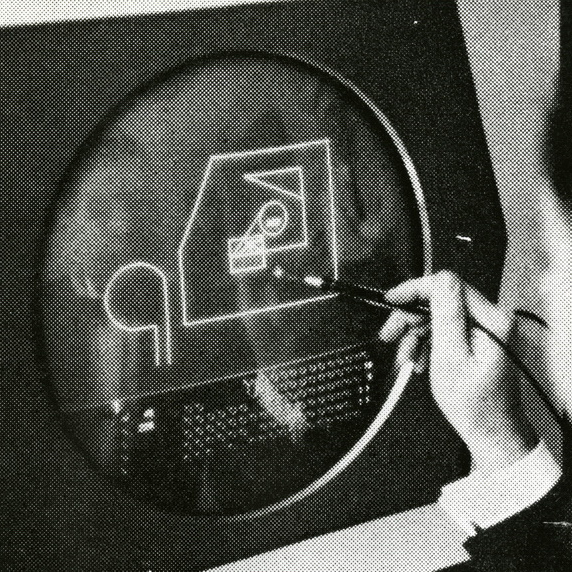
\includegraphics[width=8cm]{figuras/figura-1}}
		}{
			\Fonte{http://i0.wp.com/www.designleap.org/wp-content/uploads/2014/06/Sketchpad-Ivan-Sutherland-1963.jpg?resize=572\%2C572}
		}	
	\end{figure}
	\nocite{figura1}
	
Com o avanço resultado da criação dos circuitos integrados, cujo uso nos microprocessadores proporcionou um espantoso crescimento da indústria, os computadores deixaram de ser um monopólio das grandes companhias e tornaram-se muito mais acessíveis a pessoas simples. Isso abriu várias possibilidades para o mercado de computadores pessoais, entre elas destaca-se o surgimento das primeiras placas gráficas produzidas pela IBM (\acrlong{IBM}).

    \begin{figure}[h!]
		\centering
		\Caption{\label{fig:exemplo-2} Placa gráfica denominada Color Graphics Adapter produzida nos anos 80 pela IBM.}	
		\UNIFORfig{}{
			\fbox{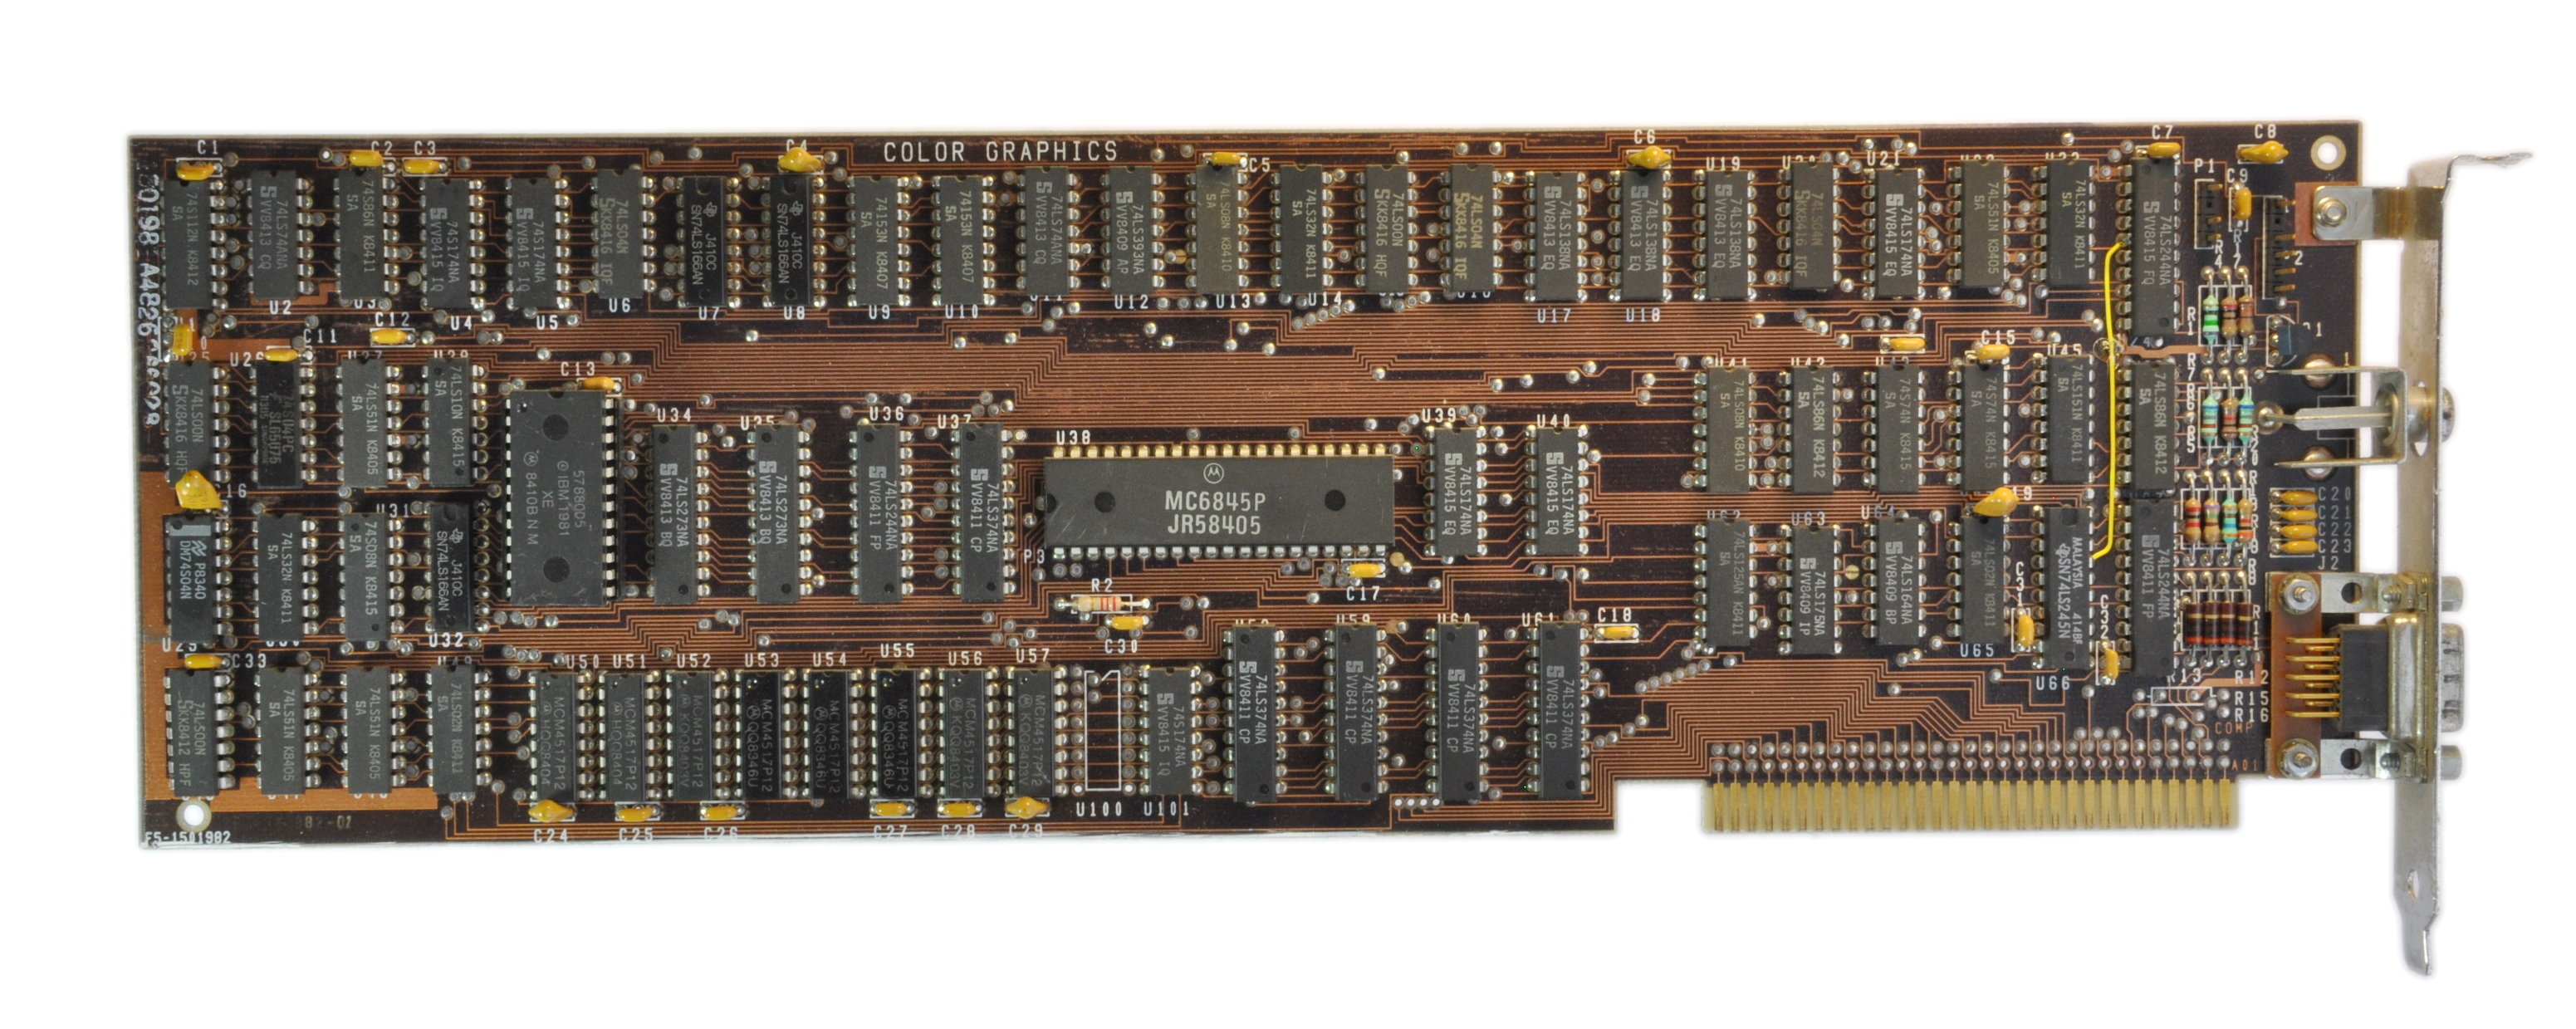
\includegraphics[width=15cm]{figuras/figura-2}}
		}{
			\Fonte{https://upload.wikimedia.org/wikipedia/commons/5/55/IBM\_Color\_Graphics\_Adapter.jpg}
		}	
	\end{figure}
	\nocite{figura2}
	
Como a indústria de jogos eletrônicos tinha mais recursos para explorar devido às melhorias de hardware disponíveis, vários jogos começaram a se destacar no mercado. Entre eles os mais marcantes para a popularização do uso de tecnologia de computação gráfica tridimensional foram lançados pela empresa id Software na década de 90. O primeiro sendo Wolfenstein 3D (que na realidade utilizava o modo 7 do Super NES (\acrlong{NES}) para emular a ambientação tridimensional) que definiu o padrão para jogos no gênero de tiro em primeira pessoa em 3D e o segundo sendo Doom que fazia uso de renderização com perspectiva 3D em tempo real por meio de software proprietário desenvolvido pela própria id Software voltado para produção com destino a computadores que utilizavam o sistema operacional da Microsoft (\acrshort{MS-DOS}).

    \begin{figure}[h!]
		\centering
		\Caption{\label{fig:exemplo-3} No lado esquerdo percebe-se que Doom fazia uso de 3D real enquanto no lado direito Wolfenstein posicionava imagens 2D em diferentes camadas para simular a profundidade tridimensional.}	
		\UNIFORfig{}{
			\fbox{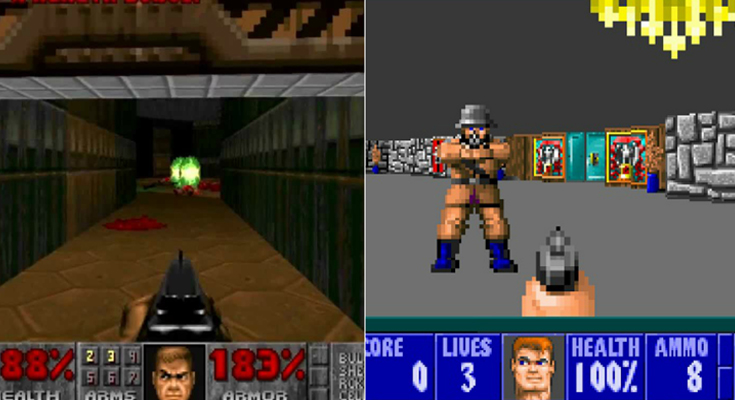
\includegraphics[width=13cm]{figuras/figura-3}}
		}{
			\Fonte{https://www.retrorefurbs.com/wolfenstein-vs-doom-the-battle-of-the-first-person-shooters/}
		}
	\end{figure}
	\nocite{figura3}
	
Paralelo ao cenário desses jogos \cite{openGLBook}, a Silicon Graphics (\acrshort{SGI}), uma companhia especializada em computação gráfica 3D e líder de mercado na época, trabalhava no lançamento open source da Open Graphics Library (\acrshort{OpenGL}), uma API (\acrlong{API}) padronizada multiplataforma de processamento de gráficos de computador em tempo real que rapidamente dominou o mercado, e que era uma derivação de outra biblioteca proprietária da mesma empresa, a IRIS GL (\acrlong{IRIS GL}). 

Vendo uma oportunidade de mercado, a Microsoft logo agiu e comprou a empresa RenderMorphics, criadora da \acrshort{API} Reality Lab, que teve o nome alterado para Direct3D e foi distribuido como um SDK (\acrlong{SDK}) conhecido como DirectX \cite{openGLBook}, acabando por se tornar o concorrente direto da \acrshort{OpenGL}. Essa rivalidade no final das contas acabou sendo benéfica tanto para o mercado de jogos eletrônicos quanto para os seus consumidores, já que acelerou o desenvolvimento de novas tecnologias que exploravam ao máximo o potencial do hardware disponível.
	
Mais adiante, em 1999, a empresa NVIDIA foi responsável for trazer mais uma inovação ao mercado, a "primeira GPU" (\acrlong{GPU}) foi como ficou conhecida a placa gráfica GeForce 256, que fazia uso de uma tecnologia chamada T\&L (\acrlong{T&L}) que basicamente movia os cálculos de transformação e iluminação de vértices da CPU (\acrlong{CPU}) para a \acrshort{GPU}. Isso permitia uma maior velocidade em operações matemáticas de ponto flutuante. Então nos próximos anos o que se viu foi um crescimento exponencial de performance de \acrshort{GPU} para renderização em tempo real.

    \begin{figure}[h!]
        \Caption{\label{fig:1} Hardware da placa gráfica da NVIDIA.}
        \begin{subfigure}{0.55\textwidth}
        \UNIFORfig{}{
			\fbox{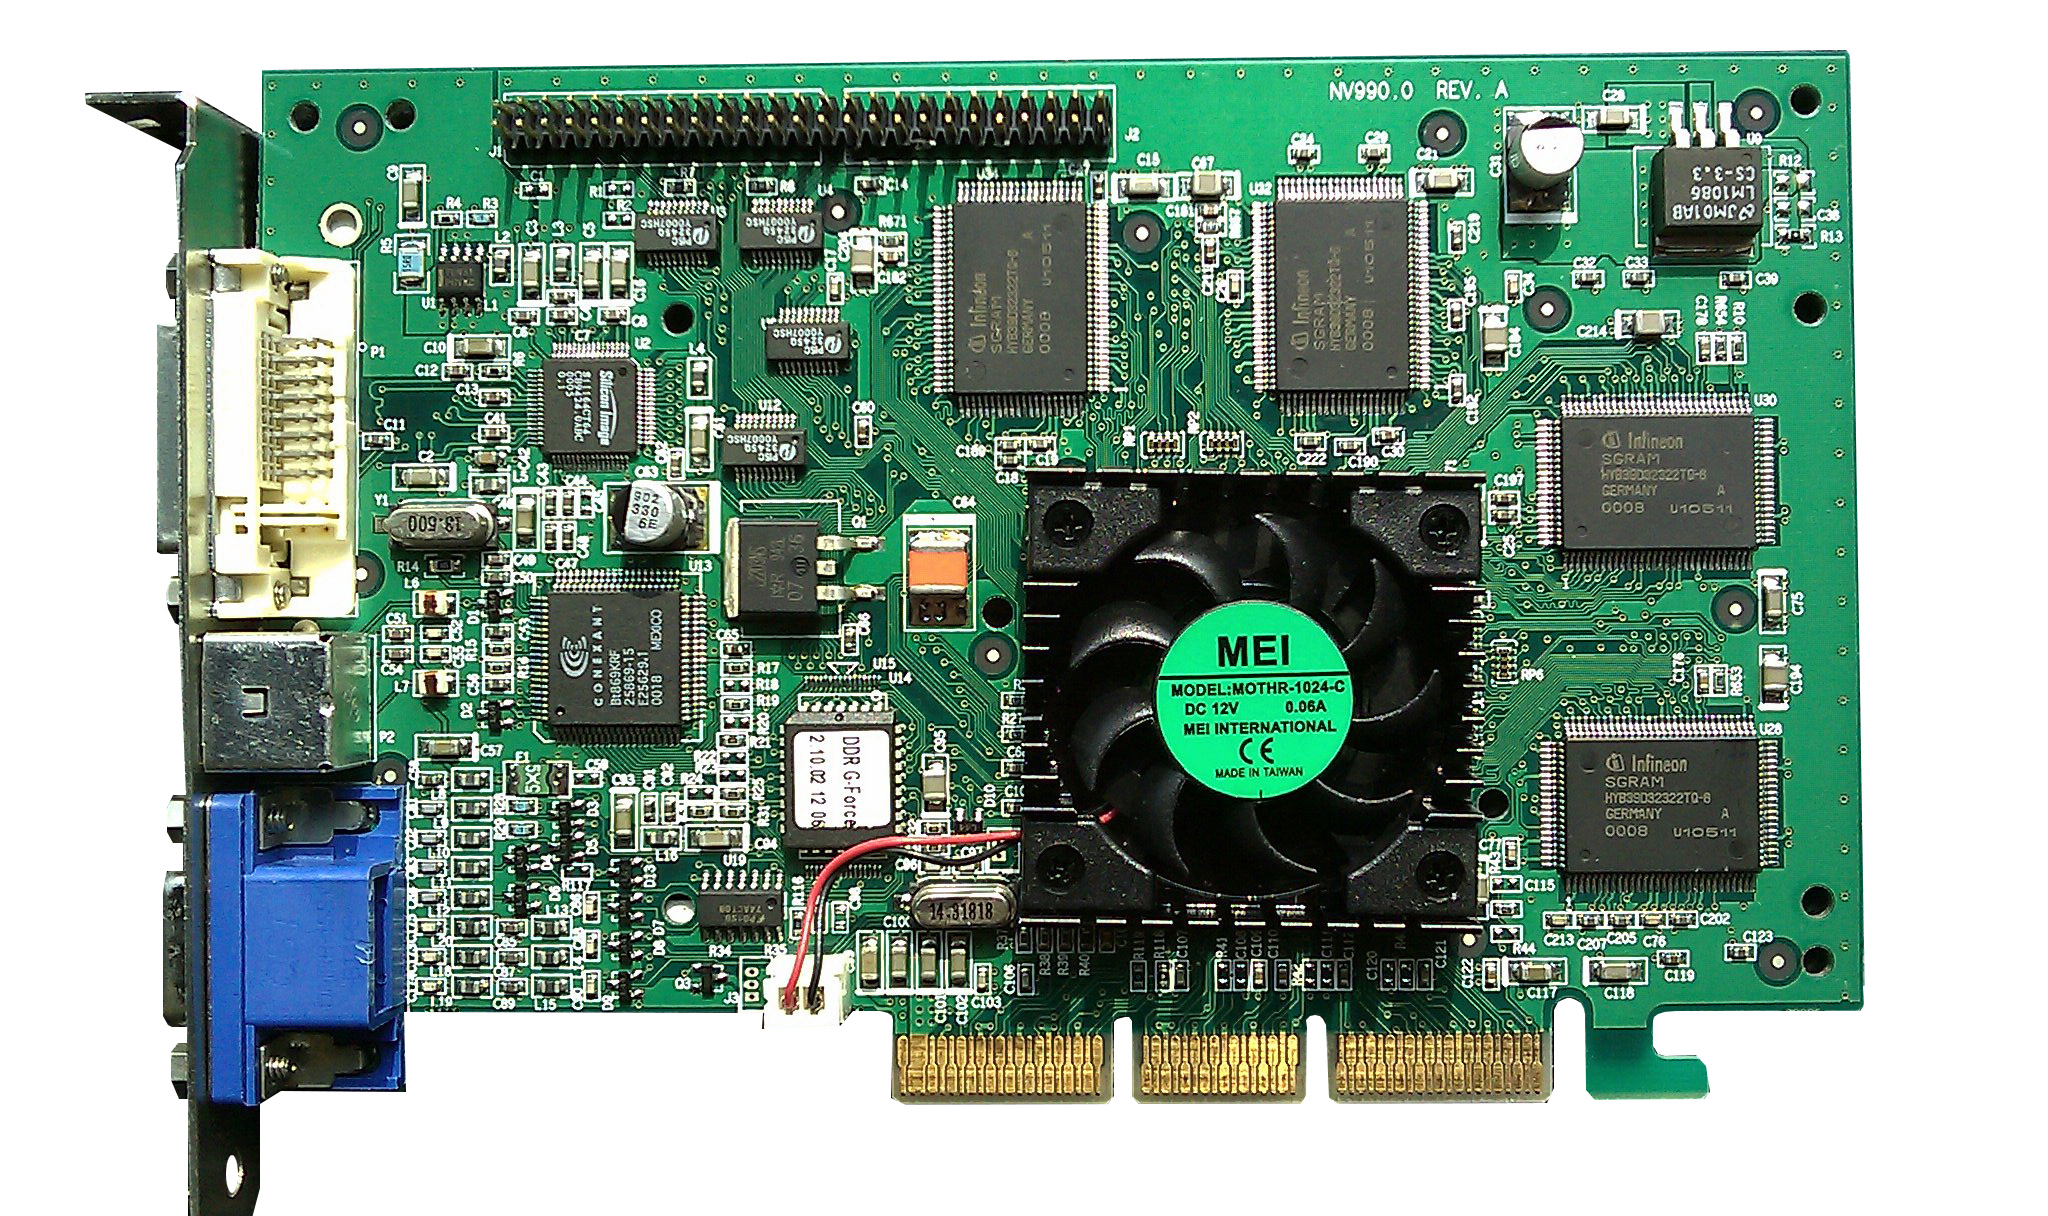
\includegraphics[width=\linewidth]{figuras/fig-a}}
		}{
		    \caption{GeForce 256} \label{fig:1a}
		}
		\nocite{figura4a}
        \end{subfigure}%
        \hspace*{\fill}
        \begin{subfigure}{0.35\textwidth}
        \UNIFORfig{}{
			\fbox{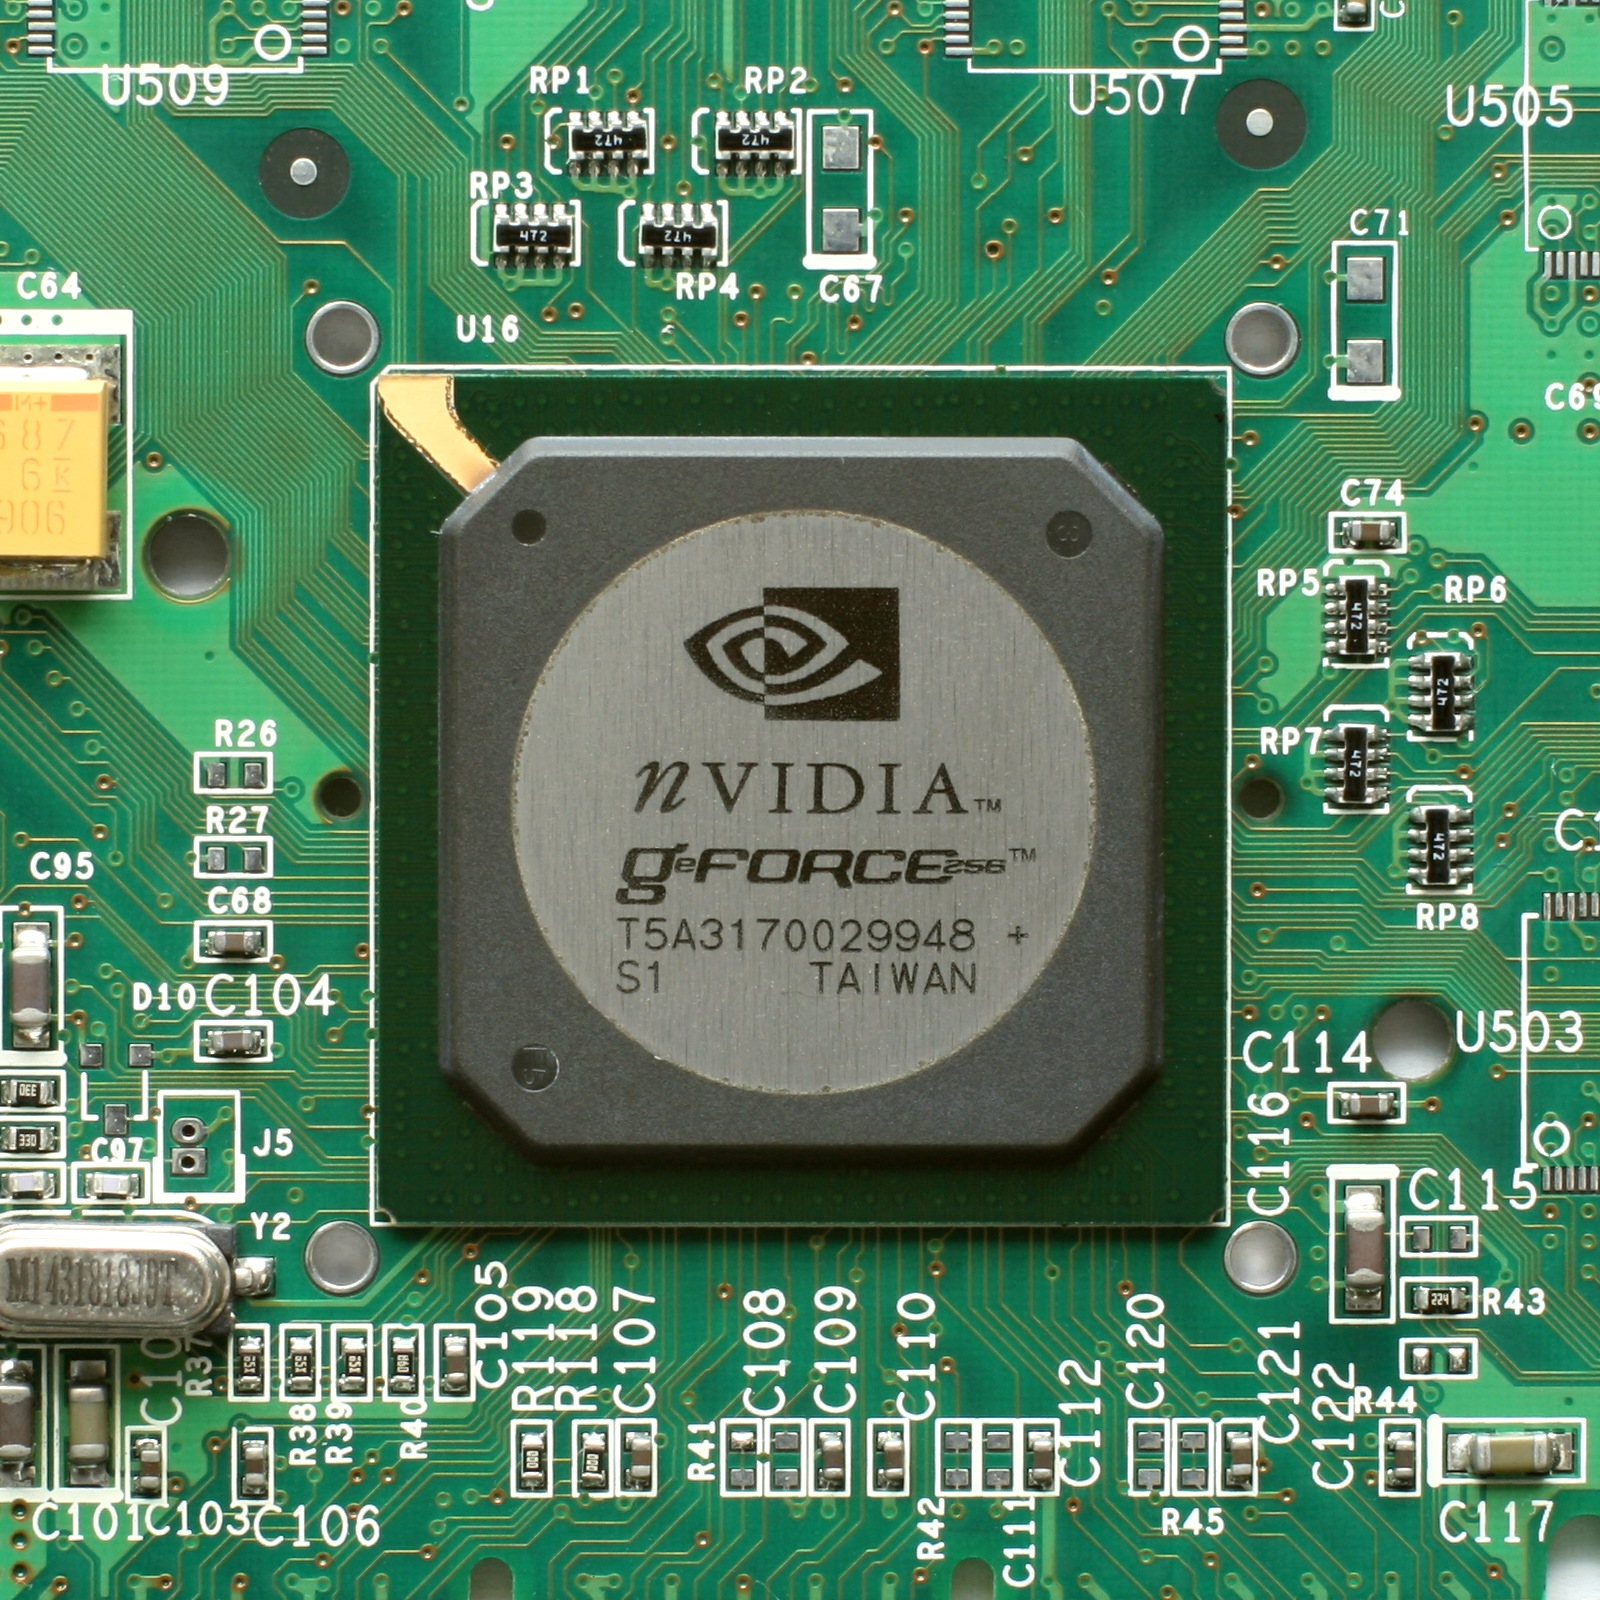
\includegraphics[width=\linewidth]{figuras/fig-b}}
		}{
		    \caption{GPU da GeForce 256} \label{fig:1b}
		}
		\nocite{figura4b}
        \end{subfigure}
		{
			\Fonte{https://upload.wikimedia.org/wikipedia/commons}
		}
	\end{figure}
	
Até então shaders eram bem vistos e utilizados por melhorar a performance eliminando carga de trabalho excessiva da \acrshort{CPU}, porém sua programação era difícil por causa da sintaxe semelhante à programação em Assembly.

\section{Fundamentação Teórica B}
\label{sec:fundamentacao-teorica-b}

Integer non lacinia magna. Aenean tempor lorem tellus, non sodales nisl commodo ut. Proin mattis placerat risus sit amet laoreet. Praesent sapien arcu, maximus ac fringilla efficitur, vulputate faucibus sem. Donec aliquet velit eros, sit amet elementum dolor pharetra eget. Integer eget mattis libero. Praesent ex velit, pulvinar at massa vel, fermentum dictum mauris. Ut feugiat accumsan augue, et ultrices ipsum euismod vitae

Nunc ac pretium dui. Mauris aliquam dapibus nulla ac mattis. Aenean non tortor volutpat, varius lectus vitae, accumsan nibh. Cras pretium vestibulum enim, id ullamcorper tortor ultrices non. Integer sodales viverra faucibus. Curabitur at dui lacinia, rhoncus lacus at, blandit metus. Integer scelerisque non enim quis ornare.

\lipsum[13]

	\begin{table}[h!]	
		\centering
		\Caption{\label{tab:exemplo-3} Duis faucibus, enim quis tincidunt pellentesque, nisl leo varius nulla, vitae tempus dui mauris ac ante purus lorem}		
		\UNIFORtab{}{
			\begin{tabular}{cll}
				\toprule
				Ranking & Exon Coverage & Splice Site Support \\
				\midrule \midrule
				E1 & Complete coverage by a single transcript & Both splice sites\\
				E2 & Complete coverage by more than a single transcript & Both splice sites\\
				E3 & Partial coverage & Both splice sites\\
				E4 & Partial coverage & One splice site\\
				E5 & Complete or partial coverage & No splice sites\\
				E6 & No coverage & No splice sites\\
				\bottomrule
			\end{tabular}
		}{
		\Fonte{Elaborado pelo autor}
	}
	\end{table}

Duis faucibus, enim quis tincidunt pellentesque, nisl leo varius nulla, vitae tempus dui mauris ac ante. Quisque purus lorem, pharetra sit amet lobortis eu, vehicula vitae purus. Ut varius, erat nec vehicula elementum, risus est tempus justo, nec vulputate augue leo egestas metus.

\lipsum[14]

	\begin{table}[h!]	
		\centering
		\Caption{\label{tab:exemplo-5} Etiam molestie, nulla a egestas aliquet, velit augue congue metus}		
		\UNIFORtab{}{
			\begin{tabular}{ccll}
				\toprule
				Quisque & pharetra & tempus & vulputate \\
				\midrule \midrule
				E1 & Complete coverage by a single transcript & Both splice sites\\
				E2 & Complete coverage by more than a single transcript & Both splice sites\\
				E3 & Partial coverage & Both splice sites & Both \\
				E4 & Partial coverage & One splice site & Both \\
				E5 & Complete or partial coverage & No splice sites & Both\\
				E6 & No coverage & No splice sites\\
				\bottomrule
			\end{tabular}
		}{
		\Fonte{Elaborado pelo autor}
	}
	\end{table}
	
	%como usar as siglas e abreviações
	%\acrlong{MIT}
	\acrlong{MIT}

\begin{alineascomponto}
	\item Integer non lacinia magna. Aenean tempor lorem tellus, non sodales nisl commodo ut
	\item Proin mattis placerat risus sit amet laoreet. Praesent sapien arcu, maximus ac fringilla efficitur, vulputate faucibus sem. Donec aliquet velit eros, sit amet elementum dolor pharetra eget
	\item Integer eget mattis libero. Praesent ex velit, pulvinar at massa vel, fermentum dictum mauris. Ut feugiat accumsan augue, et ultrices ipsum euismod vitae
	\begin{subalineascomponto}
		\item Integer non lacinia magna. Aenean tempor lorem tellus, non sodales nisl commodo ut
		\item Proin mattis placerat risus sit amet laoreet.
	\end{subalineascomponto}
\end{alineascomponto}